\begin{itemize}
\item[(1)]
\begin{itemize}
\item[(a)]
$$E_1 = \begin{bmatrix}
1 & 0 & 0 \\
-1 & 1 & 0 \\
0 & 0 & 1
\end{bmatrix}, E_2 = \begin{bmatrix}
1 & 0 & 0 \\
0 & 1 & 0 \\
-1 & 0 & 1
\end{bmatrix}, E_3 = \begin{bmatrix}
1 & 0 & 0 \\
0 & 1 & 0 \\
0 & -2 & 1
\end{bmatrix}$$
$$E_4 = \begin{bmatrix}
1 & 0 & 0 \\
0 & 1 & -1 \\
0 & 0 & 1
\end{bmatrix}, E_5 = \begin{bmatrix}
1 & 0 & -1 \\
0 & 1 & 0 \\
0 & 0 & 1
\end{bmatrix}$$
\item[(b)]
$$P = E_5E_4E_3E_2E_1$$
$$= \begin{bmatrix}
1 & 0 & -1 \\
0 & 1 & 0 \\
0 & 0 & 1
\end{bmatrix}\begin{bmatrix}
1 & 0 & 0 \\
0 & 1 & -1 \\
0 & 0 & 1
\end{bmatrix}\begin{bmatrix}
1 & 0 & 0 \\
0 & 1 & 0 \\
0 & -2 & 1
\end{bmatrix}\begin{bmatrix}
1 & 0 & 0 \\
0 & 1 & 0 \\
-1 & 0 & 1
\end{bmatrix}\begin{bmatrix}
1 & 0 & 0 \\
-1 & 1 & 0 \\
0 & 0 & 1
\end{bmatrix}$$
$$= \begin{bmatrix}
1 & 0 & -1 \\
0 & 1 & 0 \\
0 & 0 & 1
\end{bmatrix}\begin{bmatrix}
1 & 0 & 0 \\
0 & 1 & -1 \\
0 & 0 & 1
\end{bmatrix}\begin{bmatrix}
1 & 0 & 0 \\
0 & 1 & 0 \\
0 & -2 & 1
\end{bmatrix}\begin{bmatrix}
1 & 0 & 0 \\
-1 & 1 & 0 \\
-1 & 0 & 1
\end{bmatrix}$$
$$= \begin{bmatrix}
1 & 0 & -1 \\
0 & 1 & 0 \\
0 & 0 & 1
\end{bmatrix}\begin{bmatrix}
1 & 0 & 0 \\
0 & 1 & -1 \\
0 & 0 & 1
\end{bmatrix}\begin{bmatrix}
1 & 0 & 0 \\
-1 & 1 & 0 \\
1 & -2 & 1
\end{bmatrix}$$
$$= \begin{bmatrix}
1 & 0 & -1 \\
0 & 1 & 0 \\
0 & 0 & 1
\end{bmatrix}\begin{bmatrix}
1 & 0 & 0 \\
-2 & 3 & -1 \\
1 & -2 & 1
\end{bmatrix} = \begin{bmatrix}
0 & 2 & -1 \\
-2 & 3 & -1 \\
1 & -2 & 1
\end{bmatrix}$$
$$PM = \begin{bmatrix}
0 & 2 & -1 \\
-2 & 3 & -1 \\
1 & -2 & 1
\end{bmatrix}\begin{bmatrix}
1 & 0 & 2 & 1 & 5 \\
1 & 1 & 5 & 2 & 7 \\
1 & 2 & 8 & 4 & 12
\end{bmatrix} = \begin{bmatrix}
1 & 0 & 2 & 0 & 2 \\
0 & 1 & 3 & 0 & -1 \\
0 & 0 & 0 & 1 & 3
\end{bmatrix}$$
\end{itemize}
\item[(2)]
\begin{itemize}
\item[(a)]
$$\begin{bmatrix}
\begin{array}{cccc|c}
1 & 2 & 1 & 1 & 0 \\
3 & 0 & 0 & 4 & 0 \\
1 & -4 & -2 & -2 & 0
\end{array}
\end{bmatrix} \rightarrow\rightarrow \begin{bmatrix}
\begin{array}{cccc|c}
1 & 2 & 1 & 1 & 0 \\
0 & -6 & -3 & 1 & 0 \\
0 & -6 & -3 & -3 & 0
\end{array}
\end{bmatrix}$$
$$ \rightarrow \begin{bmatrix}
\begin{array}{cccc|c}
1 & 2 & 1 & 1 & 0 \\
0 & 1 & 1/2 & -1/6 & 0 \\
0 & -6 & -3 & -3 & 0
\end{array}
\end{bmatrix} \rightarrow \begin{bmatrix}
\begin{array}{cccc|c}
1 & 2 & 1 & 1 & 0 \\
0 & 1 & 1/2 & -1/6 & 0 \\
0 & 0 & 0 & -4 & 0
\end{array}
\end{bmatrix}$$
$$\rightarrow \begin{bmatrix}
\begin{array}{cccc|c}
1 & 2 & 1 & 1 & 0 \\
0 & 1 & 1/2 & -1/6 & 0 \\
0 & 0 & 0 & 1 & 0
\end{array}
\end{bmatrix}\rightarrow\rightarrow \begin{bmatrix}
\begin{array}{cccc|c}
1 & 2 & 1 & 0 & 0 \\
0 & 1 & 1/2 & 0 & 0 \\
0 & 0 & 0 & 1 & 0
\end{array}
\end{bmatrix}$$
$$\rightarrow \begin{bmatrix}
\begin{array}{cccc|c}
1 & 0 & 0 & 0 & 0 \\
0 & 1 & 1/2 & 0 & 0 \\
0 & 0 & 0 & 1 & 0
\end{array}
\end{bmatrix}$$
For arbitrary $x_3$, then $x_4 = 0, x_2 = -x_3/2, x_1 = 0$.
\item[(b)]
$$\begin{bmatrix}
\begin{array}{cccc|c}
1 & 2 & 1 & 1 & 1 \\
3 & 0 & 0 & 4 & 1 \\
1 & -4 & -2 & -2 & 0
\end{array}
\end{bmatrix} \rightarrow\rightarrow \begin{bmatrix}
\begin{array}{cccc|c}
1 & 2 & 1 & 1 & 1 \\
0 & -6 & -3 & 1 & -2 \\
0 & -6 & -3 & -3 & -1
\end{array}
\end{bmatrix}$$
$$ \rightarrow \begin{bmatrix}
\begin{array}{cccc|c}
1 & 2 & 1 & 1 & 1 \\
0 & 1 & 1/2 & -1/6 & 1/3 \\
0 & -6 & -3 & -3 & -1
\end{array}
\end{bmatrix} \rightarrow \begin{bmatrix}
\begin{array}{cccc|c}
1 & 2 & 1 & 1 & 1 \\
0 & 1 & 1/2 & -1/6 & 1/3 \\
0 & 0 & 0 & -4 & 1
\end{array}
\end{bmatrix}$$
$$\rightarrow \begin{bmatrix}
\begin{array}{cccc|c}
1 & 2 & 1 & 1 & 1 \\
0 & 1 & 1/2 & -1/6 & 1/3 \\
0 & 0 & 0 & 1 & -1/4
\end{array}
\end{bmatrix}\rightarrow\rightarrow \begin{bmatrix}
\begin{array}{cccc|c}
1 & 2 & 1 & 0 & 5/4 \\
0 & 1 & 1/2 & 0 & 7/24 \\
0 & 0 & 0 & 1 & -1/4
\end{array}
\end{bmatrix}$$
$$\rightarrow \begin{bmatrix}
\begin{array}{cccc|c}
1 & 0 & 0 & 0 & 1/2 \\
0 & 1 & 1/2 & 0 & 7/24 \\
0 & 0 & 0 & 1 & -1/4
\end{array}
\end{bmatrix}$$
For arbitrary $x_3$, $x_4 = -1/4$, $x_2 = 7/24 - x_3/2, x_1 = 2/3$.
\item[(c)]
$$\begin{bmatrix}
\begin{array}{cccc|c}
1 & 2 & 1 & 1 & 0 \\
3 & 0 & 0 & 4 & 2 \\
1 & -4 & -2 & -2 & 2
\end{array}
\end{bmatrix} \rightarrow\rightarrow \begin{bmatrix}
\begin{array}{cccc|c}
1 & 2 & 1 & 1 & 0 \\
0 & -6 & -3 & 1 & 2 \\
0 & -6 & -3 & -3 & 2
\end{array}
\end{bmatrix}$$
$$ \rightarrow \begin{bmatrix}
\begin{array}{cccc|c}
1 & 2 & 1 & 1 & 0 \\
0 & 1 & 1/2 & -1/6 & -1/3 \\
0 & -6 & -3 & -3 & 2
\end{array}
\end{bmatrix} \rightarrow \begin{bmatrix}
\begin{array}{cccc|c}
1 & 2 & 1 & 1 & 0 \\
0 & 1 & 1/2 & -1/6 & -1/3 \\
0 & 0 & 0 & -4 & 0
\end{array}
\end{bmatrix}$$
$$\rightarrow \begin{bmatrix}
\begin{array}{cccc|c}
1 & 2 & 1 & 1 & 0 \\
0 & 1 & 1/2 & -1/6 & -1/3 \\
0 & 0 & 0 & 1 & 0
\end{array}
\end{bmatrix}\rightarrow\rightarrow \begin{bmatrix}
\begin{array}{cccc|c}
1 & 2 & 1 & 0 & 0 \\
0 & 1 & 1/2 & 0 & -1/3 \\
0 & 0 & 0 & 1 & 0
\end{array}
\end{bmatrix}$$
$$\rightarrow \begin{bmatrix}
\begin{array}{cccc|c}
1 & 0 & 0 & 0 & 2/3 \\
0 & 1 & 1/2 & 0 & -1/3 \\
0 & 0 & 0 & 1 & 0
\end{array}
\end{bmatrix}$$
For arbitrary $x_3$, $x_4 = 0$, $x_2 = -1/3 - x_3/2, x_1 = 2/3$.
\end{itemize}
\item[(3)]
For arbitrary $x_2, x_3, x_4$, $x_1 = 3 - x_2 - 2x_3 + x_4$
\item[(4)]
$$E_1 = \begin{bmatrix}
1 & 0 \\
-1 & 1
\end{bmatrix}, E_2 = \begin{bmatrix}
1 & -4 \\
0 & 1
\end{bmatrix}, E_3 = \begin{bmatrix}
1 & 0 \\
-1 & 1
\end{bmatrix}$$
$$A^{-1} = E_3E_2E_1 = \begin{bmatrix}
1 & 0 \\
-1 & 1
\end{bmatrix}\begin{bmatrix}
1 & -4 \\
0 & 1
\end{bmatrix}\begin{bmatrix}
1 & 0 \\
-1 & 1
\end{bmatrix}$$
$$= \begin{bmatrix}
1 & 0 \\
-1 & 1
\end{bmatrix}\begin{bmatrix}
5 & -4 \\
-1 & 1
\end{bmatrix} = \begin{bmatrix}
5 & -4 \\
-6 & 5
\end{bmatrix}$$
\item[(5)]
$$A = \begin{bmatrix}
1 & \\
& 2
\end{bmatrix} \rightarrow \begin{bmatrix}
1 & \\
& 1
\end{bmatrix} \Rightarrow A^{-1} = \begin{bmatrix}
1 & \\
& 1/2
\end{bmatrix} $$
$$B = \begin{bmatrix}
1 & 1 \\
& 1
\end{bmatrix} \rightarrow \begin{bmatrix}
1 & \\
& 1
\end{bmatrix} \Rightarrow B^{-1} = \begin{bmatrix}
1 & -1 \\
& 1
\end{bmatrix}$$
$$C = \begin{bmatrix}
& 1 \\
1 &
\end{bmatrix} \rightarrow \begin{bmatrix}
& 1 \\
1 &
\end{bmatrix} \Rightarrow C^{-1} = \begin{bmatrix}
& 1 \\
1 &
\end{bmatrix}$$
$$D = \begin{bmatrix}
3 & 5 \\
1 & 2
\end{bmatrix} \rightarrow \begin{bmatrix}
1 & 5/3 \\
1 & 2
\end{bmatrix} \rightarrow \begin{bmatrix}
1 & 5/3 \\
& 1/3
\end{bmatrix} \rightarrow \begin{bmatrix}
1 & 5/3 \\
& 1
\end{bmatrix} \rightarrow \begin{bmatrix}
1 & \\
& 1
\end{bmatrix}$$
$$D^{-1} = \begin{bmatrix}
1 & -5/3 \\
& 1
\end{bmatrix}\begin{bmatrix}
1 & \\
& 3
\end{bmatrix}\begin{bmatrix}
1 & \\
-1 & 1
\end{bmatrix}\begin{bmatrix}
1/3 & \\
& 1
\end{bmatrix}$$
$$= \begin{bmatrix}
1 & -5/3 \\
& 1
\end{bmatrix}\begin{bmatrix}
1 & \\
& 3
\end{bmatrix}\begin{bmatrix}
1/3 & \\
-1/3 & 1
\end{bmatrix} = \begin{bmatrix}
1 & -5/3 \\
& 1
\end{bmatrix}\begin{bmatrix}
1/3 & \\
-1 & 3
\end{bmatrix}$$
$$= \begin{bmatrix}
2 & -5 \\
-1 & 3
\end{bmatrix}$$
$$E = \begin{bmatrix}
1 & 1 \\
& 1
\end{bmatrix}\begin{bmatrix}
& 1 \\
1 &
\end{bmatrix}\begin{bmatrix}
3 & 5 \\
1 & 2
\end{bmatrix} = BCD$$
$$(BCD)^{-1} = D^{-1}C^{-1}B^{-1} = \begin{bmatrix}
2 & -5 \\
-1 & 3
\end{bmatrix}\begin{bmatrix}
& 1 \\
1 &
\end{bmatrix}\begin{bmatrix}
1 & -1 \\
& 1
\end{bmatrix}$$
$$= \begin{bmatrix}
2 & -5 \\
-1 & 3
\end{bmatrix}\begin{bmatrix}
& 1 \\
1 & -1
\end{bmatrix} = \begin{bmatrix}
-5 & 7 \\
3 & -4
\end{bmatrix}$$
\item[(6)]
$Ae_1 = \begin{bmatrix}
2 & 2
\end{bmatrix}^\top, Ae_2 = \begin{bmatrix}
-1 & 3
\end{bmatrix}^\top$

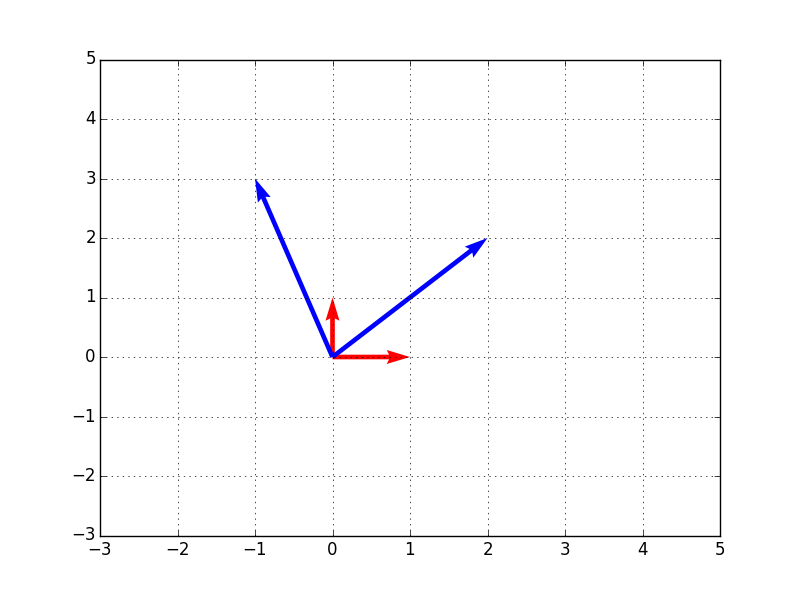
\includegraphics[scale=0.5]{fig/C1_S2_6.png}
\item[(7)]
Suppose we have a matrix $A$ in row reduced echelon form:
$$A = \begin{bmatrix}
\begin{array}{c|c|c}
& 1 & B \\
\hline
& & D
\end{array}
\end{bmatrix}$$
Suppose we can inductively reduce the submatrix $D$ with column operations such that all pivots are denoted with a 1, and all other values are 0. Then we use column operations to negate out all values in $B$. Thus, $A$ can be reduced to a matrix which only has 1's in the locations of the pivots, and all other values are 0.
\item[(8)]
\begin{itemize}
\item[(a)]
Let $A = e_{ij}$, $B = e_{k\ell}$, $E = AB$. Then
$$E_{xy} = \sum_{z = 1}^n A_{xz}B_{zy}$$
Note that if $j=k$, then
$$E_{i\ell} = \sum_{z=1}^n A_{iz}B_{z\ell} = A_{ij}B_{k\ell} = 1$$
If $j \neq k$, then $E_{i\ell} = 0$. For all other $x, y$, then $E_{xy} = 0$. 
\item[(b)]
$$I = e_{11} + e_{22} + ... + e_{nn} = \sum_{i=1}^n e_{ii}$$
\item[(c)]
Denote $A^{(k)}$ the $n \times n$ matrix where for each $i$, $A^{(k)}_{ik} = A_{ik}$, and $A^{(k)}_{ij} = A_{ij}$ for $j \neq k$. Then
$$e_{ii}Ae_{jj} = e_{ii}A^{(j)} = A_{ij}e_{ii}$$
\item[(d)]
Denote $B = e_{ij}A$. If $a = i$, then for all $b$, $B_{ab} = A_{jb}$. Otherwise, $B_{ab} = 0$.

Denote $C = Ae_{ij}$. If $b = j$, then for all $a$, $C_{ab} = A_{ai}$. Otherwise, $C_{ab} = 0$.
\end{itemize}
\item[(9)]
Let $X$ be an arbitrary matrix. Let $E_1 = I + ae_{ij}$ be a type (i) matrix. Then
$$E_1X = (I + ae_{ij}X) = X + ae_{ij}X$$
Then, if $x = i$, then for all $y$, $(E_1X)_{xy} = X_{iy} + aX_{jy}$, ie. scaling row $j$ by a and adding it to row $i$. If $x \neq i$, then for all $y$, $(E_1X)_{xy} = X_{xy}$.

Let $E_2 = I + e_{ij} + e_{ji} - e_{ii} - e_{jj}$ be a type (ii) matrix. Then
$$E_2X = (I + e_{ij} + e_{ji} - e_{ii} - e_{jj})X = X + e_{ij}X + e_{ji}X - e_{ii}X - e_{jj}X$$
Then, if $x = i$, then for all $y$, $(E_2X)_{xy} = X_{iy} + X_{jy} - X_{iy} = X_{jy}$. If $x = j$, then for all $y$, $(E_2X)_{xy} = X_{jy} + X_{iy} - X_{jy} = X_{iy}$. Otherwise, $(E_2X)_{xy} = X_{xy}$. Ie. rows $i$ and $j$ are interchanged.

Let $E_3 = I + (c - 1)e_{ii}$ be a type (iii) matrix. Then
$$E_3X = (I + (c - 1)e_{ii})X = X + (c-1)e_{ii}X$$
Then, if $x = i$, then for all $y$, $(E_3X)_{xy} = X_{iy} + (c-1)X_{iy} = cX_{iy}$. Otherwise, $(E_3X)_{xy} = X_{xy}$. Ie. row $i$ is multiplied by $c$.
\item[(10)]
Let $A'$ be the row reduced echelon form of $A$. Then there exists a set of elementary matrices $E_1, ..., E_K$ such that $E_k...E_1A = A'$. If every row of $A'$ contains a pivot, then each $A'_{ii} = 1$, and  for $ i \neq j$, $A'_{ij} = 0$, ie. $A'$ is the identity. Suppose some row $i$ of $A'$ does not contain a pivot. Then every row $\geq i$ also does not contain a pivot, and in particular each such row is a row of zeros. Therefore, $A'$ has its bottom row zero.
\item[(11)]
Consider the $2 \times 2$ matrix $A$, where
$$A = \begin{bmatrix}
a & b \\
c & d
\end{bmatrix}$$
Note that if $a = c = 0$, then $A$ is not invertible. If $c = 0$, note that $d \neq 0$ (otherwise $A$ is not invertible). Then
$$\begin{bmatrix}
a & b \\
& d
\end{bmatrix} \rightarrow \begin{bmatrix}
1 & b/a \\
& d
\end{bmatrix} \rightarrow \begin{bmatrix}
1 & b/a \\
& 1
\end{bmatrix} \rightarrow \begin{bmatrix}
1 & \\
& 1
\end{bmatrix}$$
If $a = 0$, then $b \neq 0$. Then we can swap rows 1 and 2, and proceed as above (so that 4 operations total are used). If $a \neq 0$ and $c \neq 0$, then
$$\begin{bmatrix}
a & b \\
c & d
\end{bmatrix} \rightarrow \begin{bmatrix}
1 & b/a \\
c & d
\end{bmatrix} \rightarrow \begin{bmatrix}
1 & b/a \\
& d - bc/a
\end{bmatrix} \rightarrow \begin{bmatrix}
1 & b/a \\
& 1
\end{bmatrix} \rightarrow \begin{bmatrix}
1 & \\
& 1
\end{bmatrix}$$
Note with respect to the above operations that if $ad - bc = 0$, then $A$ is not invertible. So, $A$ can be reduced to the identity in 4 operations $E_1, E_2, E_3, E_4$, where some $E_i$ may be the identity operation. Then $A^{-1} = E_4E_3E_2E_1$, so $A^{-1}$ is a product of at most 4 elementary matrices.
\item[(12)]
Suppose $A$ is not invertible. Then for some elementary row operations $E_p, E_{p-1}, ..., E_1$, $A$ has reduced echelon form $A'$ such that $E_p...E_1A = A'$, and $A'$ has a bottom row of 0s. Then $AB = (E_p...E_1)^{-1}A'B$, and furthermore $A'B$ also has a bottom row of zeros. Therefore, $AB$ is cannot row reduce to the identity matrix, and therefore $AB$ is not invertible.

Thus, if $AB$ is invertible, then $A$ is invertible. Therefore, for some set of elementary matrices, $A = E_1...E_p$. Thus, $AB = E_1...E_pB \rightarrow (AB)E_p^{-1}...E_1^{-1} = B$. Since 
$$BE_1...E_p(AB)^{-1} =(AB)E_p^{-1}...E_1^{-1}E_1...E_p(AB)^{-1} = I$$
Then $B^{-1} = E_1...E_p(AB)^{-1}$, so $B$ is invertible.
\item[(13)]
Let $A$ be a $n \times m$ matrix. Then $A^\top$ is a $m \times n$ matrix, $AA^\top$ is a $n \times n$ matrix, and
$$(AA^\top)_{ij} = \sum_{k=1}^n A_{ki}A^\top_{jk} = \sum_{k=1}^n A_{ki}A_{kj}$$
Since $(AA^\top)_{ij} = (AA^\top)_{ji}$, then $AA^\top$ is symmetric.

$$(A + A^\top)_{ij} = A_{ij} + A^\top_{ii} = A_{ij} + A_{ji}$$
Since $(A + A^\top)_{ij} = (A + A^\top)_{ji}$, then $A + A^\top$ is symmetric.
\item[(14)]
\begin{itemize}
\item[(a)] 
Let $A$ be a $n \times m$ matrix and $B$ be a $m \times n$ matrix. Then
$$(B^\top A^\top)_{ij} = \sum_{k=1}^n B^\top_{ik}A^\top_{kj} = \sum_{k=1}^n B_{ki}A_{jk} = (AB)_{ji} = ((AB)^\top)_{ij}$$

And, $((A^\top)^\top)_{ij} = (A^\top)_{ji} = A_{ij}$.
\item[(b)]
$$A^\top(A^{-1})^\top = (A^{-1}A)^\top = I^\top = I$$
Thus, $(A^{-1})^\top = (A^\top)^{-1}$.
\end{itemize}
\item[(15)]
If $A$ is symmetric and invertible, then
$$(A^{-1})^\top = (A^\top)^{-1} = A^{-1}$$
Thus $A^{-1}$ is symmetric.
\item[(16)]
Suppose $AB$ is symmetric. Then
$$AB = (AB)^\top = B^\top A^\top = BA$$
Suppose $AB = BA$. Then
$$(AB)^\top = (BA)^\top = A^\top B^\top = AB$$
Thus $AB$ is symmetric.
\item[(17)]
Suppose $AX = BX$ for arbitrary $X$. Then $(A - B)X = 0$. Consider the standard column vectors $e_1, ..., e_n$, where $e_i$ has a 1 in the $i$th position as its only nonzero entry. For $e_i$, then for all $j$, $0 = ((A - B)e_i)_j = (A - B)_{ji} = A_{ji} - B_{ji} \rightarrow A_{ji} = B_{ji}$. Thus, $A = B$.
\item[(18)]
\begin{itemize}
\item[(a)] Suppose $AX = B$ has two distinct solutions $X_1, X_2$. Then $A(X_1 - X_2) = AX_1 - AX_2 = 0$, and for all $c \in \mathbb{R}$, $A(cX_1 - cX_2) = 0$. Thus, $A(X_1 + cX_1 - cX_2) = B \rightarrow X_1 + cX_1 - cX_2$ is also a solution. Therefore, $AX = B$ has infinitely many solutions.
\item[(b)]
Suppose $A = m \times n$ matrix, and let
$$X = \begin{bmatrix}
x_1 + y_1i \\
\vdots \\
x_n + y_ni
\end{bmatrix}$$
where at least one $y_i \neq 0$. Then
$$B_j = \sum_{k=1}^n A_{jk}X_k = \sum_{k=1}^n A_{jk}(x_k + y_ki)$$
Since $B_j$ is real, then
$$\sum_{k=1}^n A_{jk}y_{k} = 0$$
The above equation is satisfied when each $y_{k} = 0$. Therefore,
$$X = \begin{bmatrix}
x_1 \\
\vdots \\
x_n
\end{bmatrix}$$
is also a solution for $AX = B$.
\end{itemize}
\item[(19)]
Suppose $A$ is a $m \times 1$ matrix. Then trivially the row reduced echelon form $A'$ of $A$ solely of zeros (if $A = 0$), otherwise $A'$ has a pivot in the first row. Suppose for all $m \times n - 1$ matrices that its corresponding row reduced echelon form is uniquely determined. Suppose now that $A$ is a $m \times n$ matrix, with distinct row reduced echelon forms $B$ and $C$. Note that $A = [A' | A"], B = [B' | B"]$ and $C = [C' | C"]$, where $A', B', C'$ are $m \times n - 1$ matrices, and $A", B", C"$ are $m \times 1$ matrices. Thus, $B', C'$ are row reduced echelon forms of $A'$, and in particular $B' = C'$. So, $B" \neq C"$: in particular for some $i$, $B"_i \neq C"_i$. Consider $AX = 0$. Then $BX = CX = 0$. So, we have
$$0 = \sum_{k=1}^n B_{ik}X_k = \sum_{k=1}^n C_{ik}X_k$$
Since for $1 \leq k \leq n-1$, $B_{ik} = C_{ik}$, then
$$0 = B_{in}X_n = C_{in}X_n \rightarrow (B_{in} - C_{in})X_n = 0$$
Since $B_{in} \neq C_{in}$, then $X_n = 0$. Therefore, $B"$ and $C"$ must contain a pivot, and since $B' = C'$ the pivot must be in the same location. But then all other entries of $B"$ and $C"$ must be 0. Thus, $B" = C"$, and by contradiction $B = C$.
\end{itemize}
